% fig_architecture.tex — Five-layer × four-function SAMBP architecture matrix
% Compile: pdflatex fig_architecture
\documentclass[tikz,border=4pt]{standalone}
\usepackage{tikz}
\usetikzlibrary{matrix,positioning,fit,backgrounds,arrows.meta,shapes.geometric}

\begin{document}
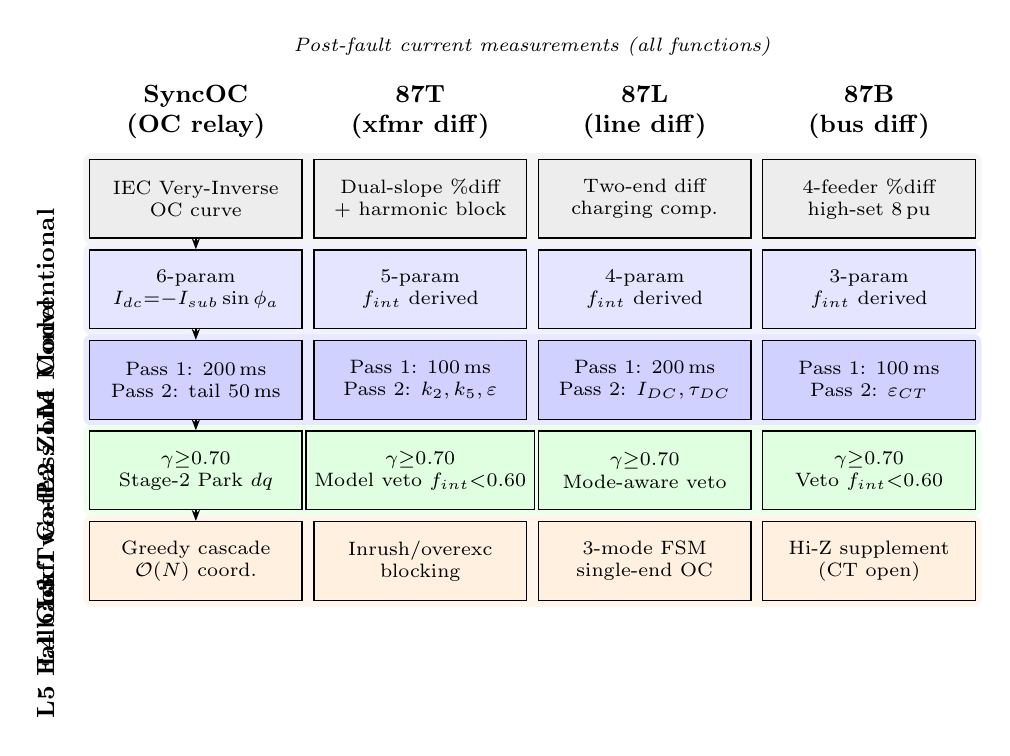
\begin{tikzpicture}[
  font=\small,
  layerlabel/.style={rotate=90,font=\small\bfseries,align=center},
  colhead/.style={font=\small\bfseries,align=center,minimum width=2.7cm},
  cell/.style={draw,minimum width=2.7cm,minimum height=1.0cm,align=center,
               fill=white,font=\scriptsize,inner sep=3pt,line width=0.5pt},
  layer1/.style={cell,fill=gray!14},
  layer2/.style={cell,fill=blue!10},
  layer3/.style={cell,fill=blue!18},
  layer4/.style={cell,fill=green!12},
  layer5/.style={cell,fill=orange!12},
  arr/.style={-{Stealth[length=4pt]},line width=0.5pt},
]

% ---- Column headers ---------------------------------------------------------
\node[colhead] (hOC)  at (0,0)    {SyncOC\\(OC relay)};
\node[colhead] (h87T) at (2.85,0) {87T\\(xfmr diff)};
\node[colhead] (h87L) at (5.70,0) {87L\\(line diff)};
\node[colhead] (h87B) at (8.55,0) {87B\\(bus diff)};

% ---- Layer 1: Conventional Baseline ----------------------------------------
\node[layer1] (L1OC)  at (0,-1.1)   {IEC Very-Inverse\\OC curve};
\node[layer1] (L1T)   at (2.85,-1.1){Dual-slope \%diff\\+ harmonic block};
\node[layer1] (L1L)   at (5.70,-1.1){Two-end diff\\charging comp.};
\node[layer1] (L1B)   at (8.55,-1.1){4-feeder \%diff\\high-set 8\,pu};

% ---- Layer 2: Zone Model ----------------------------------------------------
\node[layer2] (L2OC)  at (0,-2.25)   {6-param\\$I_{dc}{=}{-}I_{sub}\sin\phi_a$};
\node[layer2] (L2T)   at (2.85,-2.25){5-param\\$f_{int}$ derived};
\node[layer2] (L2L)   at (5.70,-2.25){4-param\\$f_{int}$ derived};
\node[layer2] (L2B)   at (8.55,-2.25){3-param\\$f_{int}$ derived};

% ---- Layer 3: Two-Pass LM ---------------------------------------------------
\node[layer3] (L3OC)  at (0,-3.40)    {Pass 1: 200\,ms\\Pass 2: tail 50\,ms};
\node[layer3] (L3T)   at (2.85,-3.40) {Pass 1: 100\,ms\\Pass 2: $k_2,k_5,\varepsilon$};
\node[layer3] (L3L)   at (5.70,-3.40) {Pass 1: 200\,ms\\Pass 2: $I_{DC},\tau_{DC}$};
\node[layer3] (L3B)   at (8.55,-3.40) {Pass 1: 100\,ms\\Pass 2: $\varepsilon_{CT}$};

% ---- Layer 4: Confidence Gate -----------------------------------------------
\node[layer4] (L4OC)  at (0,-4.55)    {$\gamma{\geq}0.70$\\Stage-2 Park $dq$};
\node[layer4] (L4T)   at (2.85,-4.55) {$\gamma{\geq}0.70$\\Model veto $f_{int}{<}0.60$};
\node[layer4] (L4L)   at (5.70,-4.55) {$\gamma{\geq}0.70$\\Mode-aware veto};
\node[layer4] (L4B)   at (8.55,-4.55) {$\gamma{\geq}0.70$\\Veto $f_{int}{<}0.60$};

% ---- Layer 5: Fallback / Coordination ---------------------------------------
\node[layer5] (L5OC)  at (0,-5.70)    {Greedy cascade\\$\mathcal{O}(N)$ coord.};
\node[layer5] (L5T)   at (2.85,-5.70) {Inrush/overexc\\blocking};
\node[layer5] (L5L)   at (5.70,-5.70) {3-mode FSM\\single-end OC};
\node[layer5] (L5B)   at (8.55,-5.70) {Hi-Z supplement\\(CT open)};

% ---- Layer labels on left ---------------------------------------------------
\node[layerlabel,left=0.55cm of L1OC] (lbl1) {\textbf{L1} Conventional};
\node[layerlabel,left=0.55cm of L2OC] (lbl2) {\textbf{L2} Zone Model};
\node[layerlabel,left=0.55cm of L3OC] (lbl3) {\textbf{L3} Two-Pass LM};
\node[layerlabel,left=0.55cm of L4OC] (lbl4) {\textbf{L4} Conf. Gate};
\node[layerlabel,left=0.55cm of L5OC] (lbl5) {\textbf{L5} Fallback};

% ---- Vertical arrows within SyncOC column -----------------------------------
\foreach \from/\to in {L1OC/L2OC, L2OC/L3OC, L3OC/L4OC, L4OC/L5OC}{
  \draw[arr] (\from.south) -- (\to.north);
}

% ---- Background shading for each layer band ---------------------------------
\begin{scope}[on background layer]
  \node[fill=gray!8,  rounded corners=3pt, inner sep=2pt,
        fit=(L1OC)(L1T)(L1L)(L1B)] {};
  \node[fill=blue!5,  rounded corners=3pt, inner sep=2pt,
        fit=(L2OC)(L2T)(L2L)(L2B)] {};
  \node[fill=blue!9,  rounded corners=3pt, inner sep=2pt,
        fit=(L3OC)(L3T)(L3L)(L3B)] {};
  \node[fill=green!7, rounded corners=3pt, inner sep=2pt,
        fit=(L4OC)(L4T)(L4L)(L4B)] {};
  \node[fill=orange!8,rounded corners=3pt, inner sep=2pt,
        fit=(L5OC)(L5T)(L5L)(L5B)] {};
\end{scope}

% ---- Common input label at top ----------------------------------------------
\node[font=\scriptsize\itshape, above=0.12cm of hOC, xshift=4.27cm]
     {Post-fault current measurements (all functions)};

\end{tikzpicture}
\end{document}
